\chapter {绪论}
\label{chp:intro}

\section{选题背景}

% With the growing attention of mobile markets, Android has accounted for 85.9\% of global market share~\cite{Gartner_report}. Over 1.5 million apps were released within 2017 alone.
% Along with the booming of Android markets is the flourish of the mobile underground industry. \emph{Fake apps}, i.e., apps without official certificates, account for a major part of such underground industry.
% Specifically, we consider fake apps as those who simulate the corresponding official ones or look almost the same as their official correspondences, with ultimate goal to elicit download or manifest malicious behaviors.
% Early observation reveals fake apps come in two different forms.
% The first category is called \texttt{imitators}, a group of apps with similar names or functionalities to their official correspondences so that users are fooled to download them.
% While imitators are just similar to official apps, \texttt{imposters}~\cite{Andow2016ASO} refer to the category of apps that have exactly the same metadata with their official correspondences, for example, they may have the same names, icons, or version numbers, some of the imposters are even made by repackaging official apk files directly.
随着移动市场于近年逐渐兴起,Android系统作为一个主流的移动端操作系统也在蓬勃发展。
数据分析机构StatCounter资料显示,Android市场占有率自发布之日起就在逐年稳步增长。
截至2020年,Android系统已经占据全球移动端市场份额的74.3\%~\cite{MobileOSMktShare}。
与此同时,Android应用的数量也伴随着Android市场的蓬勃发展节节攀高。
仅Android官方的应用商店Google Play就在2017年中新上架了近一百万个可供下载的应用程序。
虽然因为各种原因,Google Play上的应用数量在2018年有所回落,但如\autoref{fig:app_number}所示,应用市场上目前仍有近三百万个可用的应用程序,Android应用市场依然充满活力~\cite{StatistaAppNumber}。

\begin{figure}[htbp]
	\centering
	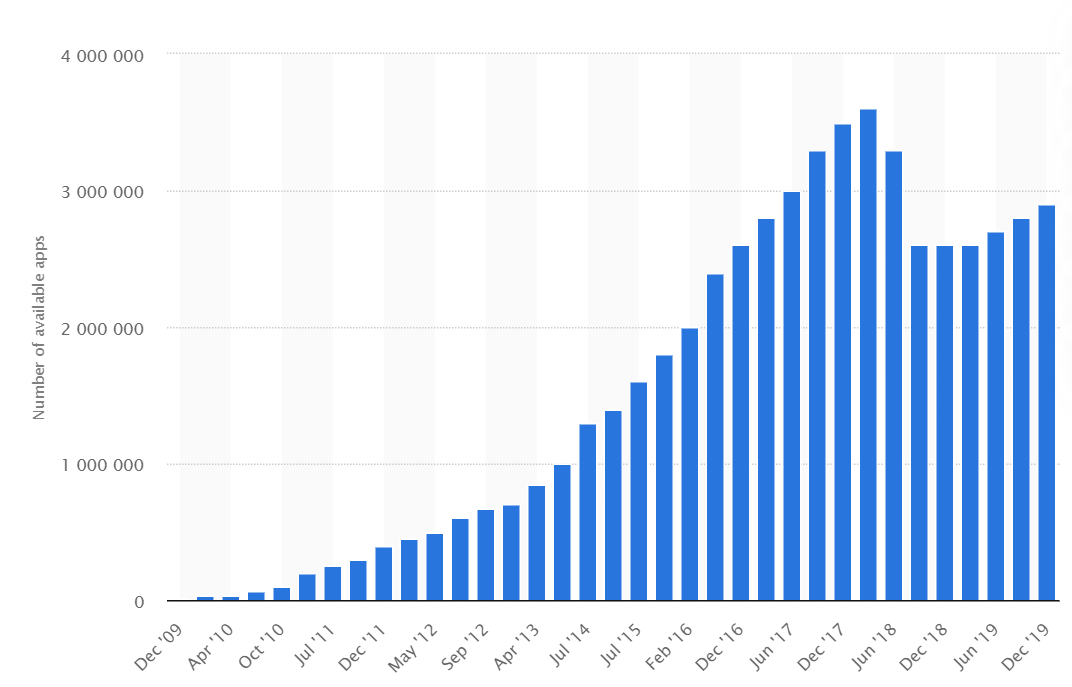
\includegraphics[width=0.9\textwidth]{./Figures/edwin-intro-app-number.png}
	\caption{Google Play 应用商店架上应用总数变化趋势}
	\label{fig:app_number}
\end{figure}

伴随着应用数量爆发式增长的,还有欣欣向荣的移动黑灰产。
黑灰产是以侵害用户、原应用作者或其他第三方利益为手段,凭此或通过其他可疑方式牟利的产业。
现阶段已知的移动黑灰产包括恶意应用的编写与传播产业、重打包应用的制作产业和在应用市场上提供批量虚假评价的产业。
据上述定义,\emph{仿冒应用}也是移动黑灰产业链中的一环。
本文提及的仿冒应用指代模仿市面上热门的应用、甚至外观与热门应用相差无几的移动应用,其目的是诱导用户下载以赚取流量,甚至是窃取用户信息、触发有害行为从而盈利。
根据的前期观察,本文发现仿冒应用以两种不同的形式出现。
第一类为\texttt{模仿应用},这类应用具有和原版热门应用相似的外观(比如名字、图标等),诱导用户下载。
而第二类---\texttt{高仿应用}~\cite{Andow2016ASO, luo2016repackage},已不单单是与原应用``相似''了,这类应用采用和原应用一模一样的外观,乃至连版本号都相同,其中的部分应用就是直接通过对原应用重打包做成的。

% Such fake apps pose significant problems to not only the official developers' interest but also the end users' right.
% For example, when users try to search an app for installation in market, multiple fake apps with similar names or icons will be retrieved at the same time.
% As a result, the user experience of app searching and downloading is greatly affected by the fake apps in real world.
这些仿冒应用不仅大大损害了原应用开发者的利益,也侵犯了用户的权益。
可以假设一个普遍场景:当用户尝试通过应用市场搜索安装一个应用,应用市场往往会返回多个无论是名字或是图标都十分相像的结果。在未有明确指引的情况下,用户十分有可能安装一个仿冒应用。
即使用户最后删除了仿冒应用,并重新装上原版应用,也浪费了时间和人力成本。
而前人研究~\cite{Zhou2012DissectingAM}显示,应用中的某些恶意行为可被自动触发。
万一用户下载的仿冒应用中包含此类恶意行为,将会对用户造成更大的损害。
可见,仿冒应用严重影响用户搜索与下载应用时的安全和体验。

% Even worse, as the doorsill to develop an app has been set low, the cost to develop a fake app is much lower than what it takes to develop a desktop program, providing an ideal hotbed for the underground industry to thrive on~\cite{wasserman2010software}. Moreover, the flexibility of Android app implementation~\cite{storydroid} contributes the fake apps' complexity.
一方面,随着开发移动应用的门槛逐渐下降,开发一个仿冒应用的成本已经远低于开发一个桌面级应用所需的成本,为地下产业涌入移动端发展提供了绝佳的温床~\cite{wasserman2010software}。
另一方面,移动应用功能在实现上的灵活性~\cite{storydroid}也增加了仿冒应用的复杂度,让分析移动应用变得更加困难。

\section{研究现状}
尽管如今仿冒应用随处可见,业界和学术界对仿冒应用和他们的生态却依然知之甚少——他们有何共同特征、数量多少、迭代速度如何、以及他们如何规避应用市场检测等问题依然有待解答。
据本文的前期调研,目前还未有任何关于仿冒应用或其生态系统的研究。
因此,本节将介绍现有针对其他移动黑灰产业的相关研究,分析各产业或研究与仿冒应用的关联。

% \subsection{Empirical study on grayware}
\subsection{针对灰色应用的实证研究}
% Andow et al.~\cite{Andow2016ASO} proposed a study of grayware, in which 9 types of greyware are defined and triaged from data retrieved from google play. We referred the definition on \textit{imposter} from this article.
Andow等人针对灰色应用的研究~\cite{Andow2016ASO}从Google Play应用商店中采集了多个应用样本。
该研究将样本分类,定义出了9种不同的灰色应用。
灰色应用指并非具有明显的恶意行为,但应用意图存疑、又或是会向系统申请过多权限的应用程序。
灰色应用不是恶意应用,但由于其盈利方式可疑,可将其归入移动黑灰产内。
本文中对\texttt{高仿应用}的定义参照了该文献的内容。

% \subsection{Empirical studies on malware ecosystem}
\subsection{针对恶意应用生态系统的研究}
% 46 malware samples on various platforms are dissected to gain understanding on their incentive system as in a survey conducted by Felt et al.~\cite{Felt2011ASO}. Meanwhile, several strategies are proposed by them to defend again these type of malware.
% Zhou and Jiang~\cite{Zhou2012DissectingAM} gathered over 1,200 malware samples across major Android malware families, systematically characterizing their different natures including installation methods, activation mechanisms and how the payload is carried out.
% These researches help expand practitioners' horizon in terms of malicious app's behavior, but the insight they provide may not suit fake app identification well.
恶意程序自桌面时代起直到如今的移动互联网时代,一直是软工与安全领域的研究重点。
在Felt主导的一次研究~\cite{Felt2011ASO}中,研究人员仔细剖析了来自多个不同平台的46个恶意程序样本以了解这些样本的激励机制。该篇文献也揭示了这些样本的运行机制和行为策略,为后人抵御此类恶意行为提供参考。
另外,Zhou和Jiang~\cite{Zhou2012DissectingAM}搜集了来自多个主要恶意应用家族的、超过1,200个恶意应用样本,并系统性地描绘了这批样本的不同性质,包括其安装手段、激活机制和其如何执行有效负载(实现恶意行为);在另一篇著作~\cite{zhou2012hey}中,他们提出了名为DroidRanger的系统,成功地从5个应用市场的204,040个应用中找出了211个恶意应用。

这类研究帮助了业界人员拓宽视野,使得业界人员对恶意应用的行为更加了解。
然而根据前文定义,仿冒应用与恶意应用并不相同,针对仿冒应用的专门研究依然有必要。

% \subsection{Repackage detection}
\subsection{针对重打包应用检测研究}
\label{sec:repackaging}
% Prior work on repackage detection generally falls into five categories.
% The first one is based on apps' \textit{instruction sequences}, which uses fuzzy hashing techniques to extract the digest of apps, then calculates similarity between every two digests~\cite{DroidMOSS,Zheng2013DroidAnalyticsA}.
% The second one is based on \textit{semantic information}.
% CLANdroid~\cite{CLANdroid} detects similar apps through analyzing five semantic anchors (e.g., identifiers and Android APIs).
% The third kind leverages \textit{lib detection} methods.
% CodeMatch~\cite{CodeMatch} filters out libraries used in apps then compares the hash of their remnant.
% Wukong~\cite{Wukong} detects repackage apps in two steps, but that it processes the second step by using a counting-based code clone detection approach, instead of hash.
% ViewDroid~\cite{ViewDroid} picks out repackage apps by rebuilding and comparing the viewgraph of different apps, belongs to the forth kind which makes use of \textit{visualizes information}.
% The fifth kind applies \textit{graph theory} on measuring app similarity.
% DNADroid~\cite{DNADroid} calculate apps' similarity based on program dependency graph (PDG), while AnDarwin~\cite{AnDarwin} builds semantic vectors with PDG extracted from every methods.
% Centroid~\cite{Centroid} even constructs 3D-control-flow-graph (3D-CFG) for each method in an app and see how alike the centroid in different apps are.
重打包指恶意开发者对原应用解包、篡改内容之后再将应用重新打包的技术。
重打包应用侵害了应用原作者的知识产权,因此也属于移动黑灰产业范畴。
针对重打包检测的前人研究大致可划分为五个类别:

第一类基于应用\textit{指令序列}。这类方法使用模糊哈希的方法提取出应用的摘要信息,通过比对两两应用之间的摘要信息获得应用之间的相似度~\cite{DroidMOSS, Zheng2013DroidAnalyticsA}。
第二类凭借\textit{语义信息}比对应用。CLANdroid~\cite{CLANdroid}通过分析五种语义特征点(比如代码中的标识符和调用到的Android API等),以检测相似应用。
第三类利用\textit{第三方库}进行检测。CodeMatch~\cite{CodeMatch}筛选出应用中使用的第三方库代码后,计算并比对剩余部分代码的哈希值,获取不同应用的相似程度。
Wukong~\cite{Wukong}也分两步检测重打包应用,但与CodeMatch相比,其第二步使用了基于计数的代码克隆检测手段,而非基于哈希的技术。
ViewDroid~\cite{ViewDroid}通过重建和比对应用的视图来筛出重打包应用,属于第四类---\textit{信息可视化}。
第五类依赖\textit{图论}衡量应用相似性。
DNADroid~\cite{DNADroid}基于应用的程序依赖图(Program Dependency Graph, PDG)比对应用,而AnDarwin~\cite{AnDarwin}则用从每个方法中提取的PDG构建出语义向量,再计算向量间相似度以检测重打包应用。
Centroid~\cite{Centroid}甚至为应用中的每个函数构建了三维控制流图(3-Dimensional Control Flow Graph, 3D-CFG),再将三维控制流图聚合,通过检测不同应用在控制图聚合后的质心位置判断应用间的相似程度。

% Each of these approaches has its own advantages and drawbacks, from the perspective of scalability and accuracy, which are beyond the topic in this article.
% One common they all do share, however, are that the verification step, without any exception, is based on certificate system.
% Once the illegal developers poison data with legal certificates through apps with vulnerable signature scheme, even the state of the art detecting approach can do nothing about it.
以上检测方法各有其优缺点,但在最后的验证阶段都需要使用Android安全证书对APK文件进行验证,以确定是否误判。
因此,在原版Android安全证书已知的前提下,直接用证书比对是最简洁有用的验证方式。

虽然重打包应用与仿冒应用互有重合之处,但并非所有仿冒应用都为重打包应用。
因此,要了解仿冒应用的性质和特征,只对重打包应用进行观察是不足的,需要详尽地从应用市场上收集样本后再进行探索。

\subsection{针对应用评论相关移动黑灰产的研究}
近年来,除了利用应用程序牟利以外,移动黑灰产业也开始进入应用市场评论的领域。
大量的前人工作~\cite{hernandez2019the, xie2014grouptie, zhu2014discovery, hu2019want, chen2017toward, xie2016you, hooi2016fraudar}揭示,很多应用市场都饱受虚假评论的困扰。
Rahman等人在2019年发布的关于虚假评论行为的实证研究~\cite{rahman2019art}在公开确认了这个产业链存在的同时,也揭露了该产业的行为模式、生存情况甚至是从业人员收入水平等方面的信息。
作为黑灰色产业链下游环节,虚假应用评论(即排名欺诈行为)很可能与仿冒应用相结合,为移动黑灰产从业者牟取更多利益。

\section{问题分析与研究难点}

前文的研究现状,不仅反映出移动黑灰产业是目前的研究热点之一,更反映出移动黑灰产从业人员无孔不入的特点。
为了保障正当开发者的利益与消费者的权益,学术界和工业界都需要对移动黑灰产有更全面、更深入的理解,从而更好地预防未知的威胁。
上述研究现状表明,工业界与学术界的软工、安全领域在移动黑灰产的研究上已经取得了丰富的成果,然而现有研究提供的知识仍有空缺部分,仿冒应用部分正是缺口之一。
现阶段,在缺乏仿冒应用相关研究的情况下,仿冒应用数据缺失,造成了以下问题:

1)\	\emph{无法对仿冒应用进行定量分析} \quad
目前,学术界与工业界目前对恶意应用和排名欺诈行为均有良好理解,厂家得以在实践中抵御、规避此类移动黑灰产的侵袭,这得益于前人在实证调查研究~\cite{Felt2011ASO, Zhou2012DissectingAM, zhou2012hey, rahman2019art}中提供的数据与洞见(Insight)。
然而,在仿冒应用数据缺失的情况下,相关定量分析与定性分析无法进行,无法让学术界与工业界对仿冒应用有清楚了解。
针对仿冒应用进行实证研究可以有效解决这个问题。
具体而言,可利用实证研究中的混合方法途径(Mixed-methods approaches)方法论~\cite{easterbrook2008selecting},先从工业界环境(即各应用市场)中获取大量应用,再从所获应用中进行筛选,可获得一定数量的仿冒应用,从而开展相关定量分析。

2)\	\emph{无法确定仿冒应用的性质} \quad
尽管仿冒应用在日常生活中随处可见,却少有研究者对其进行研究。
因而,仿冒应用的形态尚未明确,亦从未有前人评估仿冒应用的风险性;总结仿冒应用的发展趋势不明,无法确定这一移动黑灰产是否会更加壮大;仿冒应用的市场反馈无人探索,仿冒应用是否会与其他黑灰产业环节结合更是不得而知。
针对以上疑问,可采用实证研究的混合方法途径方法论可以通过对数据定性分析,帮助理解仿冒应用具有的性质;而相对的案例分析(Case studies)方法论~\cite{easterbrook2008selecting}则可以在案例支持下更有力地确认定性分析的发现。

综上,现时仿冒应用数据匮乏、对仿冒应用了解缺失的问题,可通过实证研究缓解。
因此,本文与犇众信息的移动安全威胁数据平台Janus~\cite{janus}合作,搜集并分析了大量应用样本,从仿冒应用特征解读和仿冒应用评论分析两方面进行了大规模实证研究,对仿冒应用作出了较为全面的剖析,填补了本领域的研究空白。
仿冒应用特征解读利用数据挖掘分析技巧,利用本研究收集到的仿冒应用数据对仿冒应用进行画像;
仿冒应用评论分析则通过收集仿冒应用在市场上获得的反馈,验证仿冒应用和排名欺诈行为的关系,进一步地提供了关于仿冒应用生态的信息。

在数据挖掘分析中,研究者通常都会遇到几点挑战:如何确定研究主体、如何收集数据、如何对数据进行有效处理;
而在排名欺诈相关研究中,如何从评论数据中有效挖掘排名欺诈行为是研究者经常要思考的问题。
故本实证研究中的难点可概括如下:

1)\	\emph{如何确定仿冒应用} \quad
仿冒应用和正版应用是相对的概念。
本文选择了市面上最热门的50个应用,再搜集其对应的仿冒应用样本。
从应用中筛选出与热门应用外观相似或是相同的样本后,本文使用Android本身自带的证书机制,将获得样本的证书信息与原版应用的证书信息进行比对,从而鉴别出仿冒的样本。

2)\	\emph{如何获得针对仿冒应用的大量数据} \quad
数据搜集是科研工作中公认的难点。
本文想要提供一次全面的研究结果,除了搜集的目标应用需要有多样性之外,也必须获得不同应用市场上的数据,增加研究的代表性。
前文提及犇众信息的移动安全威胁数据平台Janus是一个数据整合平台。该平台每天从各大Android应用市场爬取应用样本入库,免去了要针对各个市场重新定制爬虫代码的麻烦。
通过设计和实现仿冒应用收集框架\mytool,本文顺利从Janus搜寻到了近14万条数据条目作为原始数据,其中每条数据条目代表Janus从应用市场上获得的一个应用样本。

3)\	\emph{如何对大量的数据进行有效处理} \quad
数据规模和处理效率一直是一对矛盾。
由于一条数据条目代表一个应用样本,要对所有应用样本进行详尽分析,明显太耗费时间成本与计算成本;然而,如果只对样本进行简单处理,获得的分析结果就不够全面和深入。
在尽量确保分析全面性的前提下,对于每个样本,本研究只抽取8个关键信息项进行分析,以节省时间与计算成本。

4)\ \emph{如何挖掘评论中的排名欺诈行为} \quad
现有的排名欺诈挖掘工作均具有其各自的局限性,或是对数据有连续收集要求,或是要求检测者有已知的排名欺诈群体,并不能直接应用到本研究收集的数据中。
为此,本研究先后设计了基于用户行为可信度和基于评论内容重复度的两个方法。
前者规避了现有方法的局限性,后者进一步解决了大数据量带来的大运算量问题。

\section{研究方法与工作概览}

\subsection{研究方法}
前文已经提及,实证研究能够为研究主体提供画像与洞见,从而为对应方面的后续实践与研究提供建议与便利。
在软件工程领域与安全领域,已有多篇实证研究为实践工作~\cite{Felt2011ASO, Zhou2012DissectingAM, zhou2012hey, rahman2019art, wu2016ji, yang2015xin}提供知识支持。
因此,本文亦将采用实证研究方式,对仿冒应用进行探索。

实证研究是一种基本研究手段,旨在针对技术在实际应用场景下的真实状况或对应产物进行数据收集、调查与分析。
Easterbrook等人于2008年提出了面向软件工程领域的实证研究方法建议\cite{easterbrook2008selecting},为软工实证研究提供方法论指导,其中将实证研究方法论分为受控实验、案例分析、调查研究、社会学意义研究与混合方法途径等多类,分别适用于不同场景。
本文研究中使用到的是混合方法途径与案例分析,简介如下:

1)\ \emph{混合方法途径(Mixed-method approaches)} \quad
混合方法途径指结合定量分析与定性分析,对研究对象进行系统数据解读的实证研究方法。
按照实施的方式,混合方法途径可分为顺序解释策略(Sequential explanatory strategy)、顺序探索策略(Sequential exploratory strategy)与并发三角策略(Concurrent triangular strategy)三类。
其中,顺序解释策略先收集与分析定量数据,再收集和分析定性数据,以定性数据结果帮助解释定量结果;与之相反,顺序探索策略先收集与分析定性数据,再收集和分析定量数据,以定量数据结果帮助解释定性结果;并发三角策略则会同时采用不同方法,以试图确认、交叉验证或证实已有发现。
本文的特征解读部分先采用定量分析方法分析数据,再采用案例分析方法给出定性结果,使用了顺序解释策略;而后续的仿冒应用与排名欺诈关联验证先给出定性结论,再提供定量数据支持,则使用了顺序探索策略。

2)\ \emph{案例分析(Case studies)} \quad
案例分析是软件工程领域最常用的实证研究方法,完整的案例分析通过确立研究问题、选择研究案例和收集数据三步研究真实场景中出现的现象,适用于真实环境为对研究主体产生影响的因素之一、又或是实验数据时间跨度较大的场景。
对于针对某些现象的初步调查,可使用探索性案例分析(Exploratory case studies)以提出新猜想和构建理论;而验证性案例分析(Confirmatory case studies)则用于验证现存理论。
本文的案例分析既包含用于提出新猜想的探索性案例分析,亦包含验证数据画像的验证性案例分析。

\subsection{工作概览}

\begin{figure}[htbp]
	\centering
	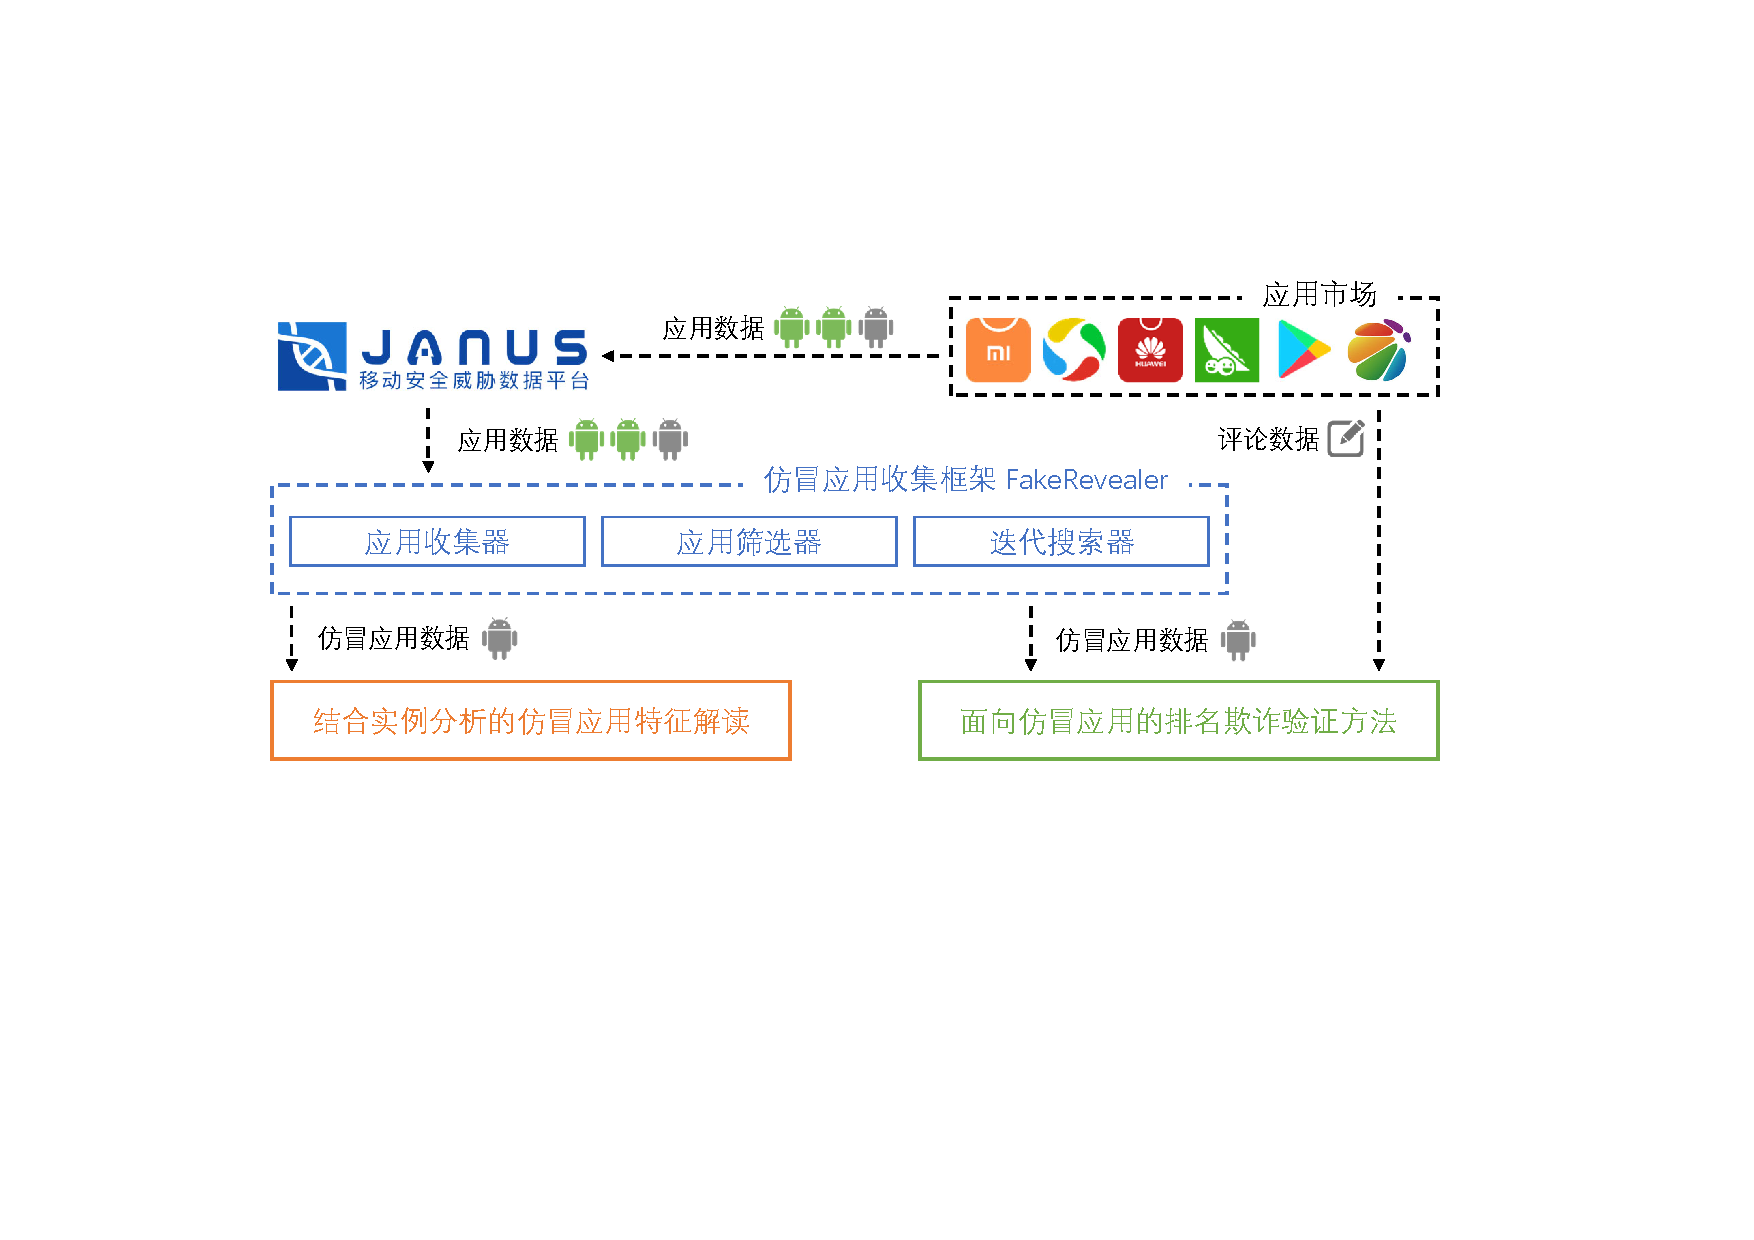
\includegraphics[width=\textwidth]{./Figures/edwin-overview}
	\caption{本文工作概览}
	\label{fig:Workflow}
	\vspace{-3mm}
\end{figure}

本节为本文工作提供概览。如\autoref{fig:Workflow}所示,本工作通过三个主要部分完成实证研究:

1)\ \emph{面向仿冒应用的收集框架\mytool } \quad
针对现有爬虫框架不能定向爬取应用的问题,本研究设计并实现了仿冒应用收集框架\mytool,以进行仿冒应用的数据收集。
数据收集主要分为两个部分:正版应用信息的收集和仿冒应用的收集。
在正版应用信息收集的部分,本文选择了50个最热门的App作为目标应用,然后手动收集了跟这些App有关的信息;
仿冒应用信息收集方面,本研究利用\mytool,通过Janus平台收集了从各个应用商店获得的大量仿冒应用样本。

2)\ \emph{结合案例分析的仿冒应用特征解读} \quad
针对移动黑灰产研究中关于仿冒应用的研究空白,本研究收集仿冒应用数据,结合案例分析,进行了首次基于Android系统仿冒应用的特征解读。
特征解读从三个视角完成,这些视角分别是仿冒的基本应用特征、影响仿冒应用数量的因素和仿冒应用的发展轨迹,由浅入深揭示仿冒应用的生态。
对应的三个案例分析除了为特征解读提供案例支持之外,还揭示了更多仿冒应用开发者的行为特征。

3)\ \emph{面向仿冒应用的排名欺诈验证方法} \quad
在这个部分,本文从第三方应用市场中随机选取一部分应用,爬取了用户对它们的所有历史评价,以检测仿冒应用与排名欺诈行为的关联。
针对前人检测研究需要先验知识或特殊数据的问题,本研究从社交媒体研究引入了用户行为可信度进行排查,避开了现有方法的局限性。
进一步地,本研究从评论内容重复率方面提出了另一创新性排查方法,解决了数据量增大带来的大运算量问题。
人工复查结果显示,两种排查方法均取得了优于现有方法的结果。


\section{本文组织结构}
本文共分为五章,环绕着本研究的数据搜集、分析过程和分析结果展开,各章节内容如下:

\fullref{chp:intro} 主要提供了本文的研究背景、相关工作、研究意义和工作概览。

\fullref{chp:background} 介绍了Android应用的构建流程、Android安全证书机制、应用市场与黑灰产业的关系和一些移动黑灰产知识。

\fullref{chp:fakerevealer} 阐述了仿冒应用收集框架\mytool 的设计缘由,说明了仿冒应用的数据收集方式并详细介绍了其中三个组件(\componentA、\componentB 和\componentC)的设计与实现,最后提供仿冒应用数据概览。

\fullref{chp:discoveries} 从多个视角分类提出并解说针对这批仿冒应用数据得到的发现。
这些视角包括仿冒应用特征、影响仿冒应用数量的因素和仿冒应用的发展轨迹,每个视角都被进一步分解成了多个不同的研究问题。
在完成每个视角的解读后,本文均从数据中挑选一个具有代表性的案例进行分析,以案例进一步深化分析结果。

\fullref{chp:feedback} 提供了面向仿冒应用的排名欺诈检测方法。
针对现有检测方法的不足,本文先后提出了两个具有创新性的方法对排名欺诈行为进行排查。
结果显示,仿冒应用与排名欺诈行为作为移动黑灰产的两个环节确实存在关联。

\fullref{chp:future} 对本文工作进行总结,并对下一步工作进行展望。
